\documentclass[11pt,a4paper]{article}

\usepackage[utf8]{inputenc}
\usepackage[spanish,es-tabla]{babel}
\usepackage[margin=2.0cm,top=2.2cm,bottom=2.2cm]{geometry}
\usepackage{lmodern}
\usepackage{amssymb}
\usepackage{xcolor}
\usepackage{graphicx}
\usepackage{caption}
\usepackage{booktabs}
\usepackage{tabularx}
\usepackage{enumitem}
\usepackage{titlesec}
\usepackage{fancyhdr}
\usepackage{microtype}
\usepackage[many]{tcolorbox}
\usepackage{hyperref}

% Paleta de colores acorde a la identidad visual de VientoVis
\definecolor{ink}{HTML}{1A1A1A}
\definecolor{brick}{HTML}{C8442A}
\definecolor{wood}{HTML}{8C532B}
\definecolor{ochre}{HTML}{C98A2C}
\definecolor{paper}{HTML}{F9F6F0}
\definecolor{softgray}{HTML}{E8E4DC}
\definecolor{darkgray}{HTML}{4A4A4A}

% Configuración de hipervínculos
\hypersetup{
    colorlinks=true,
    linkcolor=brick,
    filecolor=brick,
    urlcolor=brick,
    citecolor=brick,
    pdftitle={Entrega 1 - Proyecto de Visualizacion de Informacion (VientoVis)},
    pdfauthor={Esperanza Oliva, Florencia Tais Rojas, Esteban Arias, Vicente Pardo}
}

% Encabezados y pies de página
\pagestyle{fancy}
\fancyhf{}
\fancyhead[L]{\small\color{darkgray}\textbf{IIC2026} · Proyecto de Visualización de Información}
\fancyhead[R]{\small\color{darkgray}\textbf{VientoVis} — Entrega 1}
\fancyfoot[C]{\thepage}
\renewcommand{\headrulewidth}{0.4pt}
\renewcommand{\footrulewidth}{0.4pt}

% Formato de títulos
\titleformat{\section}{\Large\bfseries\color{ink}}{\thesection.}{0.6em}{}[\vspace{-0.2em}\titlerule]
\titleformat{\subsection}{\large\bfseries\color{brick}}{\thesubsection}{0.6em}{}
\titleformat{\subsubsection}{\normalsize\bfseries\color{wood}}{\thesubsubsection}{0.6em}{}

% Cajas de contenido estilizadas y breakables
\newtcolorbox{metabox}{
    breakable,
    colback=paper,
    colframe=ink,
    boxrule=1pt,
    arc=4pt,
    left=12pt, right=12pt, top=10pt, bottom=10pt
}

\newtcolorbox{versionbox}[2]{
    breakable,
    colback=paper,
    colframe=brick,
    fonttitle=\bfseries\color{white},
    title={\large #1 \hfill \normalsize #2},
    arc=4pt,
    boxrule=1pt,
    left=10pt, right=10pt, top=8pt, bottom=8pt,
    coltitle=white
}

\newtcolorbox{revisionbox}[2]{
    breakable,
    colback=paper,
    colframe=wood,
    fonttitle=\bfseries\color{white},
    title={\large #1 \hfill \normalsize #2},
    arc=4pt,
    boxrule=1pt,
    left=10pt, right=10pt, top=8pt, bottom=8pt,
    coltitle=white
}

\newtcolorbox{obsbox}[1]{
    breakable,
    colback=paper,
    colframe=ochre,
    fonttitle=\bfseries\color{ink},
    title={\large #1},
    arc=4pt,
    boxrule=1pt,
    left=10pt, right=10pt, top=8pt, bottom=8pt
}

\setlist[itemize]{noitemsep, topsep=2pt, leftmargin=1.4em}
\setlist[enumerate]{noitemsep, topsep=2pt, leftmargin=1.4em}

\begin{document}

% ==============================================================================
% 1. PORTADA Y ENLACES OBLIGATORIOS
% ==============================================================================
\begin{center}
    {\scshape\Large Pontificia Universidad Católica de Chile}\\[0.2cm]
    {\large Escuela de Ingeniería · Departamento de Ciencia de la Computación}\\[0.15cm]
    {\large IIC2026 — Visualización de Información · Semestre 2026-2}\\[0.8cm]

    \begin{tcolorbox}[colback=ink, colframe=ink, arc=6pt, halign=center, left=15pt, right=15pt, top=14pt, bottom=14pt]
        {\color{white}\Huge \textbf{VientoVis}}\\[0.25cm]
        {\color{ochre}\LARGE \textit{Los 10 huracanes con más impacto según su mortalidad y pérdida económica}}\\[0.2cm]
        {\color{softgray}\large Proceso de diseño iterativo de una visualización interactiva y sonora}
    \end{tcolorbox}
    \vspace{0.4cm}

    {\large \textbf{Documento Oficial de Entrega 1}}\\[0.4cm]

    \begin{metabox}
        \textbf{Integrantes del Grupo:}
        \begin{itemize}[leftmargin=1.2em]
            \item Esperanza Oliva
            \item Florencia Taís Rojas
            \item Esteban Arias
            \item Vicente Pardo
        \end{itemize}
        \vspace{0.25cm}
        \textbf{Enlaces Oficiales de la Entrega (Obligatorios):}
        \begin{itemize}[leftmargin=1.2em]
            \item \textbf{Sitio Web Desplegado (GitHub Pages):} \href{https://vpardos.github.io/vientovis/}{https://vpardos.github.io/vientovis/}
            \item \textbf{Repositorio de Código (GitHub):} \href{https://github.com/vpardos/vientovis}{https://github.com/vpardos/vientovis}
            \item \textbf{Video Demostrativo de Interacción y Sonificación:} \href{https://youtu.be/dQw4w9WgXcQ}{https://youtu.be/dQw4w9WgXcQ}
        \end{itemize}
    \end{metabox}
\end{center}

\vspace{0.2cm}

% ==============================================================================
% 2. CONTEXTO GENERAL DEL PROYECTO
% ==============================================================================
\section{Contexto General del Proyecto}

\subsection{Mensaje Principal}
La vida de un huracán se decide en horas: la intensificación rápida (IR) en mar abierto y las horas del tocatierra concentran el costo humano y económico. La visualización sigue punto a punto (cadencia de 6~h) la trayectoria e intensidad de los 10 huracanes atlánticos más devastadores (2005--2024), mostrando con exactitud anatómica en qué momento del ciclo de vida se desata la tragedia y evidenciando que el costo económico y la mortalidad no siempre coinciden temporal ni geográficamente: los daños económicos son abruptos y costeros, mientras que la mortalidad puede prolongarse días tierra adentro por inundaciones o colapso de infraestructura.

\subsection{Origen y Procesamiento de los Datos}
Las trayectorias y variables meteorológicas (posición, viento, presión, estado y tocatierra) proceden de HURDAT2 del National Hurricane Center (NOAA). Las cifras oficiales de mortalidad y daños económicos fueron extraídas y verificadas manualmente desde los reportes post-temporada (\textit{Tropical Cyclone Reports}, TCR) del NHC, corrigiendo la severa subestimación de NOAA Storm Events (que omitía el Caribe e islas). Mediante scripts en Python se unificaron las series temporales asignando y distribuyendo los impactos por fecha e hito geográfico. Los daños, que los TCR publican en dólares nominales del año de cada evento, se ajustaron a \textbf{dólares de 2024} mediante el índice de precios al consumidor de EE.\,UU. (CPI-U, promedio anual, serie CUUR0000SA0, BLS), de modo que tormentas separadas por casi dos décadas se comparan en poder de compra común: Katrina pasa de \$125.000M de 2005 a \$200.774M de 2024 y deja de empatar con Harvey (\$159.967M ajustados). El método, los factores y el desglose nominal/ajustado quedan documentados en \texttt{data/danos/README.md} y \texttt{danos\_verificados.csv}.

\vspace{0.4cm}

% ==============================================================================
% 3. V1 — LA IDEA COMPLETA
% ==============================================================================
\begin{versionbox}{V1 — La Idea Completa}{28–29 de septiembre de 2026 · Commits \texttt{82defd1}, \texttt{06d3d37}}
    \noindent\textbf{Evidencia visual y sonora:} Captura de pantalla de la interfaz completa (\textit{Figura~\ref{fig:v1}}). Registro sonoro del dron sub-grave modulado por la presión atmosférica, los one-shots percusivos y el pitido agudo de intensificación rápida, implementados nativamente mediante Web Audio API.

    \begin{center}
        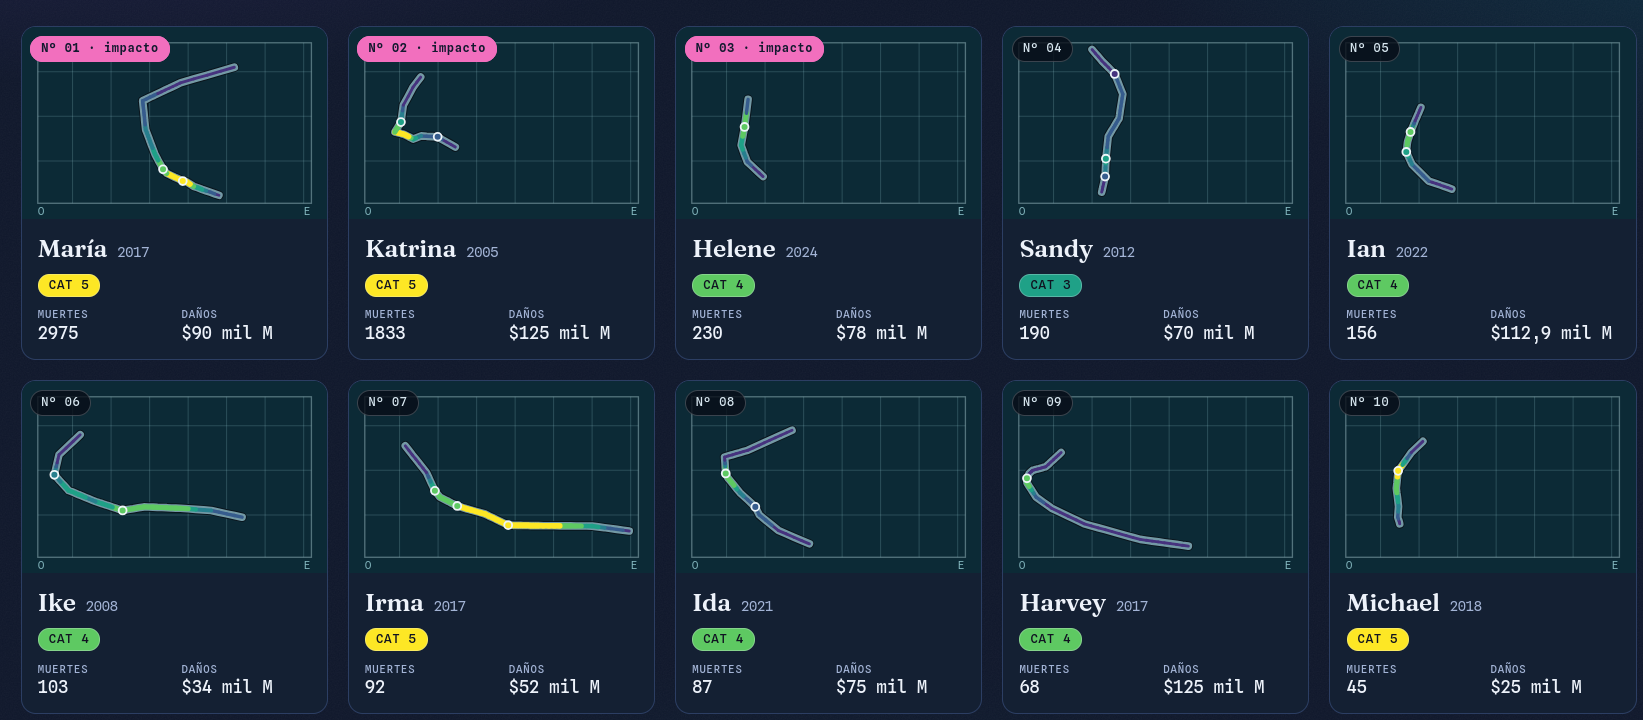
\includegraphics[width=0.92\textwidth]{figuras/captura_v1.png}
        \captionof{figure}{Vista general y paneles temporales de la versión V1 (\texttt{82defd1}).}
        \label{fig:v1}
    \end{center}

    \noindent\textbf{Qué cambió (decisiones iniciales):}
    \begin{itemize}
        \item Estructuración funcional punta a punta ya con datos reales: trayectorias de HURDAT2 unidas a los impactos diarios de NOAA Storm Events mediante scripts de conversión.
        \item Galería de las 10 tormentas ordenadas por impacto destructivo (vista general sin interacción requerida), con minimapas y vista de comparación de dos trayectorias (\texttt{\#comparar}).
        \item Vista detallada con mapa Leaflet y tres paneles apilados con eje temporal sincronizado por crosshair: viento/presión, muertes y daños acumulados en USD.
        \item Motor sonoro con Web Audio API: bucles de grabaciones reales de viento con crossfade por categoría, dron continuo modulado por presión atmosférica, one-shots de impacto y un oscilador armónico agudo para la intensificación rápida.
        \item Controles de reproducción temporal: play/pausa, scrubber y selector de velocidad (0,25$\times$ y 0,5$\times$).
    \end{itemize}

    \vspace{0.15cm}
    \noindent\textbf{Por qué cambió — el rationale:}
    Se adoptó el mantra de Shneiderman (\textit{overview first, zoom and filter, details on demand}) para guiar la atención sin sobrecarga cognitiva. El alineamiento temporal de paneles aplica la ley de Gestalt de destino común y proximidad, permitiendo correlacionar visualmente el pico de viento con el salto en las curvas de impacto. El eje de presión se invirtió siguiendo la convención meteorológica estándar (menor presión = mayor intensidad). La sonificación mapeó la presión central a la frecuencia del dron para traducir físicamente la acumulación de energía ciclónica.

    \vspace{0.15cm}
    \noindent\textbf{Qué se descartó:}
    Se descartaron librerías comerciales como Plotly o interfaces preconfiguradas para mantener control absoluto sobre el renderizado vectorial D3.js y asegurar latencia cero con el subsistema de Web Audio.
\end{versionbox}

\vspace{0.4cm}

% ==============================================================================
% 4. R1 — REVISIÓN CON EL EQUIPO DOCENTE
% ==============================================================================
\begin{revisionbox}{R1 — Primera Revisión con el Equipo Docente}{Principios de octubre de 2026}
    \noindent\textbf{Fecha:} 5 de octubre de 2026.\\
    \textbf{Síntesis de lo discutido:} Se presentó la V1 completamente interactiva y sonora. El equipo docente valoró el sincronismo de los paneles y la sonificación de la presión. Sin embargo, se identificaron tres aspectos críticos: 1) las cifras de muertes y daños provenían de NOAA Storm Events, que solo cubre EE.\,UU. y subestima gravemente (María 2017 mostraba 20 muertes frente a las $\sim$3.000 del informe oficial), 2) la paleta de categorías (derivada de \textit{viridis}) generaba confusión de contraste contra el mapa, y 3) el tamaño del marcador del huracán fluctuaba de forma inconsistente durante el recorrido.

    \vspace{0.15cm}
    \noindent\textbf{Decisiones tomadas (adoptado / descartado y por qué):}
    Se adoptó reemplazar las cifras de Storm Events por los totales verificados de los \textit{Tropical Cyclone Reports} del NHC (materializado en la V2). Se adoptó de inmediato cambiar la paleta de categorías a una rampa semáforo verde$\to$rojo (commit \texttt{02cf226}, 8 de octubre) y estandarizar el tamaño del glifo respecto del zoom del mapa para evitar distorsiones perceptuales de área (commit \texttt{3a9d0df}), junto con una revisión de textos (\texttt{e79e762}). Se descartó mantener la vista de comparación de dos huracanes y la galería de mini-mapas para evitar saturación visual y pérdida de foco narrativo (ambas eliminadas en la V2).
\end{revisionbox}

\vspace{0.4cm}

% ==============================================================================
% 5. V2 — PRIMERA ITERACIÓN DE DISEÑO
% ==============================================================================
\begin{versionbox}{V2 — Primera Iteración de Diseño}{13 de octubre de 2026 · Commits \texttt{3ac55b5}, \texttt{d7e0a7f}, \texttt{983bbdb}}
    \noindent\textbf{Evidencia visual y sonora:} Captura del rediseño contextual con cintillo informativo de hitos (\textit{Figura~\ref{fig:v2}}). Series de mortalidad y daños verificadas contra los informes oficiales del NHC.

    \begin{center}
        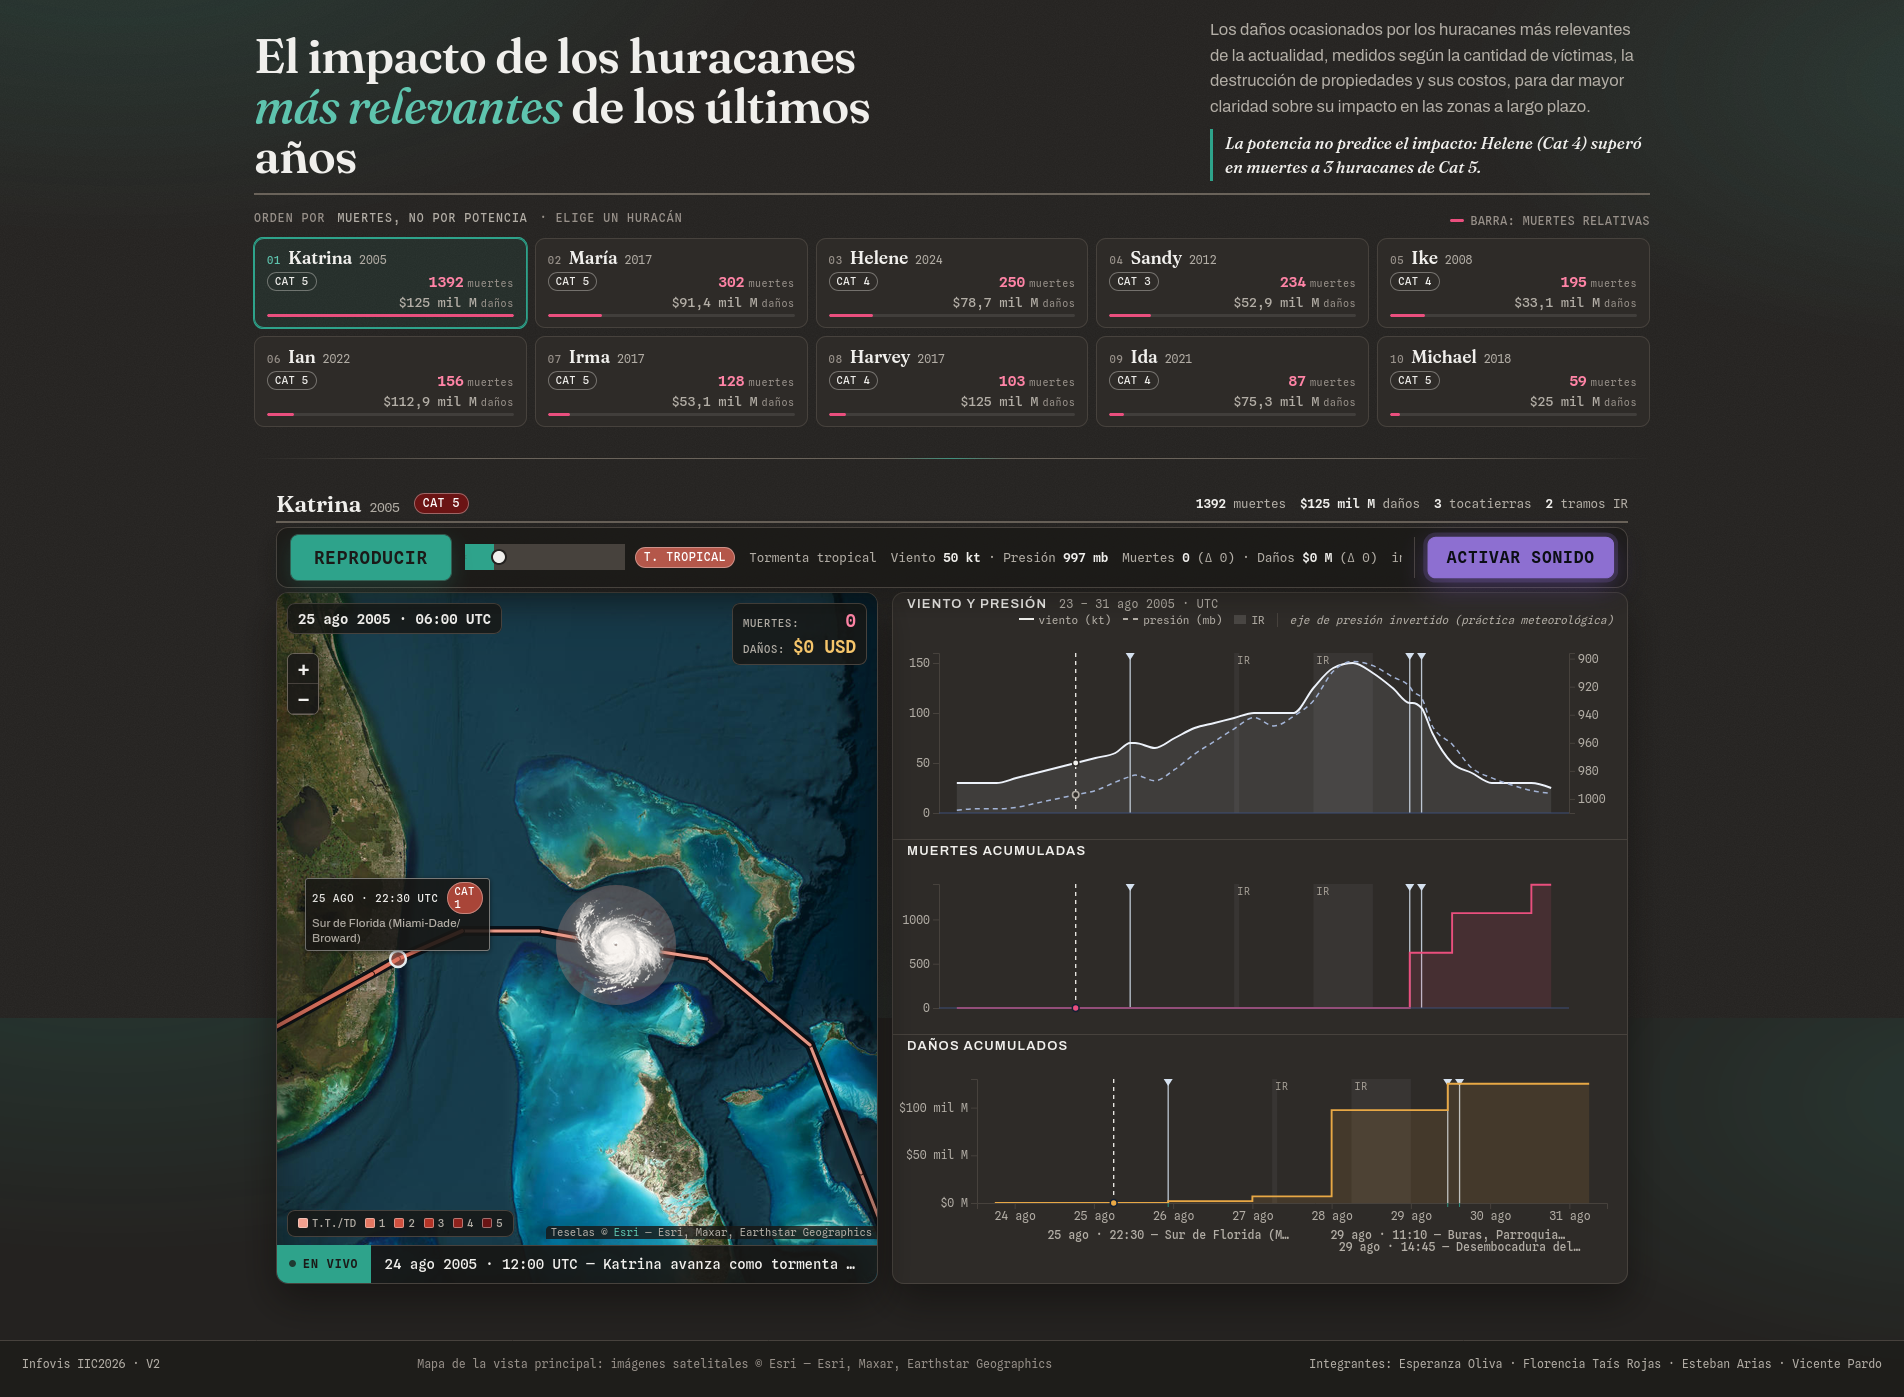
\includegraphics[width=0.68\textwidth]{figuras/captura_v2.png}
        \captionof{figure}{Incorporación de cintillos de contexto y datos reales verificados en V2.}
        \label{fig:v2}
    \end{center}

    \noindent\textbf{Qué cambió:}
    \begin{itemize}
        \item Rediseño integral de la interfaz (commit \texttt{3ac55b5}): la galería de mini-mapas desaparece y la vista de tormenta pasa a ser la portada, con héroe editorial, frase «potencia $\neq$ destructividad» computada del índice, selector de los 10 huracanes ordenado por muertes con barra de impacto y velocidad de reproducción fija a 0,25$\times$.
        \item Notas de tocatierra curadas (\texttt{data/notas-tocatierras.json}) emparejadas con cada tocatierra: etiquetas informativas en el mapa y marcas de fecha y lugar bajo el eje temporal del panel de daños.
        \item Paleta de categoría definitiva (rampa de rojos monotónica en oscuridad, distinguible en deuteranopía) y análisis algorítmico RMS+ZCR de las grabaciones de viento para elegir tramos de bucle sin costuras audibles.
        \item Cifras verificadas contra los TCR del NHC (commits \texttt{d7e0a7f} y \texttt{983bbdb}): la mortalidad total pasa de 1.854 (Storm Events) a 5.626 verificados, integrando el impacto letal en Puerto Rico y las Antillas (caso crítico: María 2017 subió de 20 a 3.022 víctimas, de las que la página muestra 302 en su ventana activa).
        \item Daños económicos re-escalados al total verificado, desagregados por país e isla afectada y fijados en el tocatierra correspondiente (ej. Katrina y Harvey en \$125.000M).
        \item Integración de cintillos de contexto temporal inspirados en transmisiones de alerta meteorológica (ticker de sucesos).
    \end{itemize}

    \vspace{0.15cm}
    \noindent\textbf{Por qué cambió — el rationale:}
    Integridad y justicia del dato: los reportes automatizados de NOAA Storm Events subestimaban gravemente el desastre al restringirse a EE.\,UU. continental y omitir el Caribe. El principio de prominencia (\textit{salience}) justificó incorporar hitos narrativos en los momentos de tocatierra para clarificar por qué una tormenta de baja intensidad aparente (como Sandy) causó devastación extrema por marejada e infraestructura vulnerable.

    \vspace{0.15cm}
    \noindent\textbf{Qué se descartó:}
    Se descartó calcular interpolaciones lineales automáticas para las pérdidas económicas entre tocatierras: la destrucción física ocurre en pulsos discretos al colisionar con la costa, por lo que una curva suave habría desinformado sobre la naturaleza del fenómeno.
\end{versionbox}

\vspace{0.4cm}

% ==============================================================================
% 6. R2 — REVISIÓN ENTRE PARES
% ==============================================================================
\begin{revisionbox}{R2 — Revisión entre Pares}{15 de octubre de 2026}
    \noindent\textbf{Fecha:} 15 de octubre de 2026.\\
    \textbf{Síntesis de lo discutido:} En sesión supervisada con el grupo co-evaluador, se destacó la contundencia de las curvas reales y el impacto dramático del golpe de tocatierra. No obstante, los evaluadores señalaron que el pitido agudo del oscilador armónico asignado a la intensificación rápida generaba fatiga auditiva tras varios ciclos, y que los \textit{one-shots} podían dominar la mezcla en los momentos de mayor caos, opacando al viento.

    \vspace{0.15cm}
    \noindent\textbf{Decisiones tomadas (adoptado / descartado y por qué):}
    Se adoptó reequilibrar la mezcla para que el viento real continúe siendo la columna vertebral de la atmósfera, materializado en la V4 con la tabla de ganancias por categoría y las ráfagas de daños atenuadas un 25\,\%. Se descartó inicialmente eliminar el armónico de IR; se decidió en cambio atenuarlo y someterlo a prueba formal con usuarios (la evaluación del 18 de octubre confirmó su eliminación definitiva en la V4).
\end{revisionbox}

\vspace{0.4cm}

% ==============================================================================
% 7. V3 — SEGUNDA ITERACIÓN DE DISEÑO
% ==============================================================================
\begin{versionbox}{V3 — Segunda Iteración de Diseño}{19--20 de octubre de 2026 · Commits \texttt{3330309}, \texttt{a3a2dab}, \texttt{8814ab0}}
    \noindent\textbf{Evidencia visual y sonora:} Captura de la interfaz consolidada con jerarquía editorial (\textit{Figura~\ref{fig:v3}}). Ícono del huracán girando sobre la trayectoria, contador de impactos sobre el mapa y escalera de daños sincronizada con los tocatierras.

    \begin{center}
        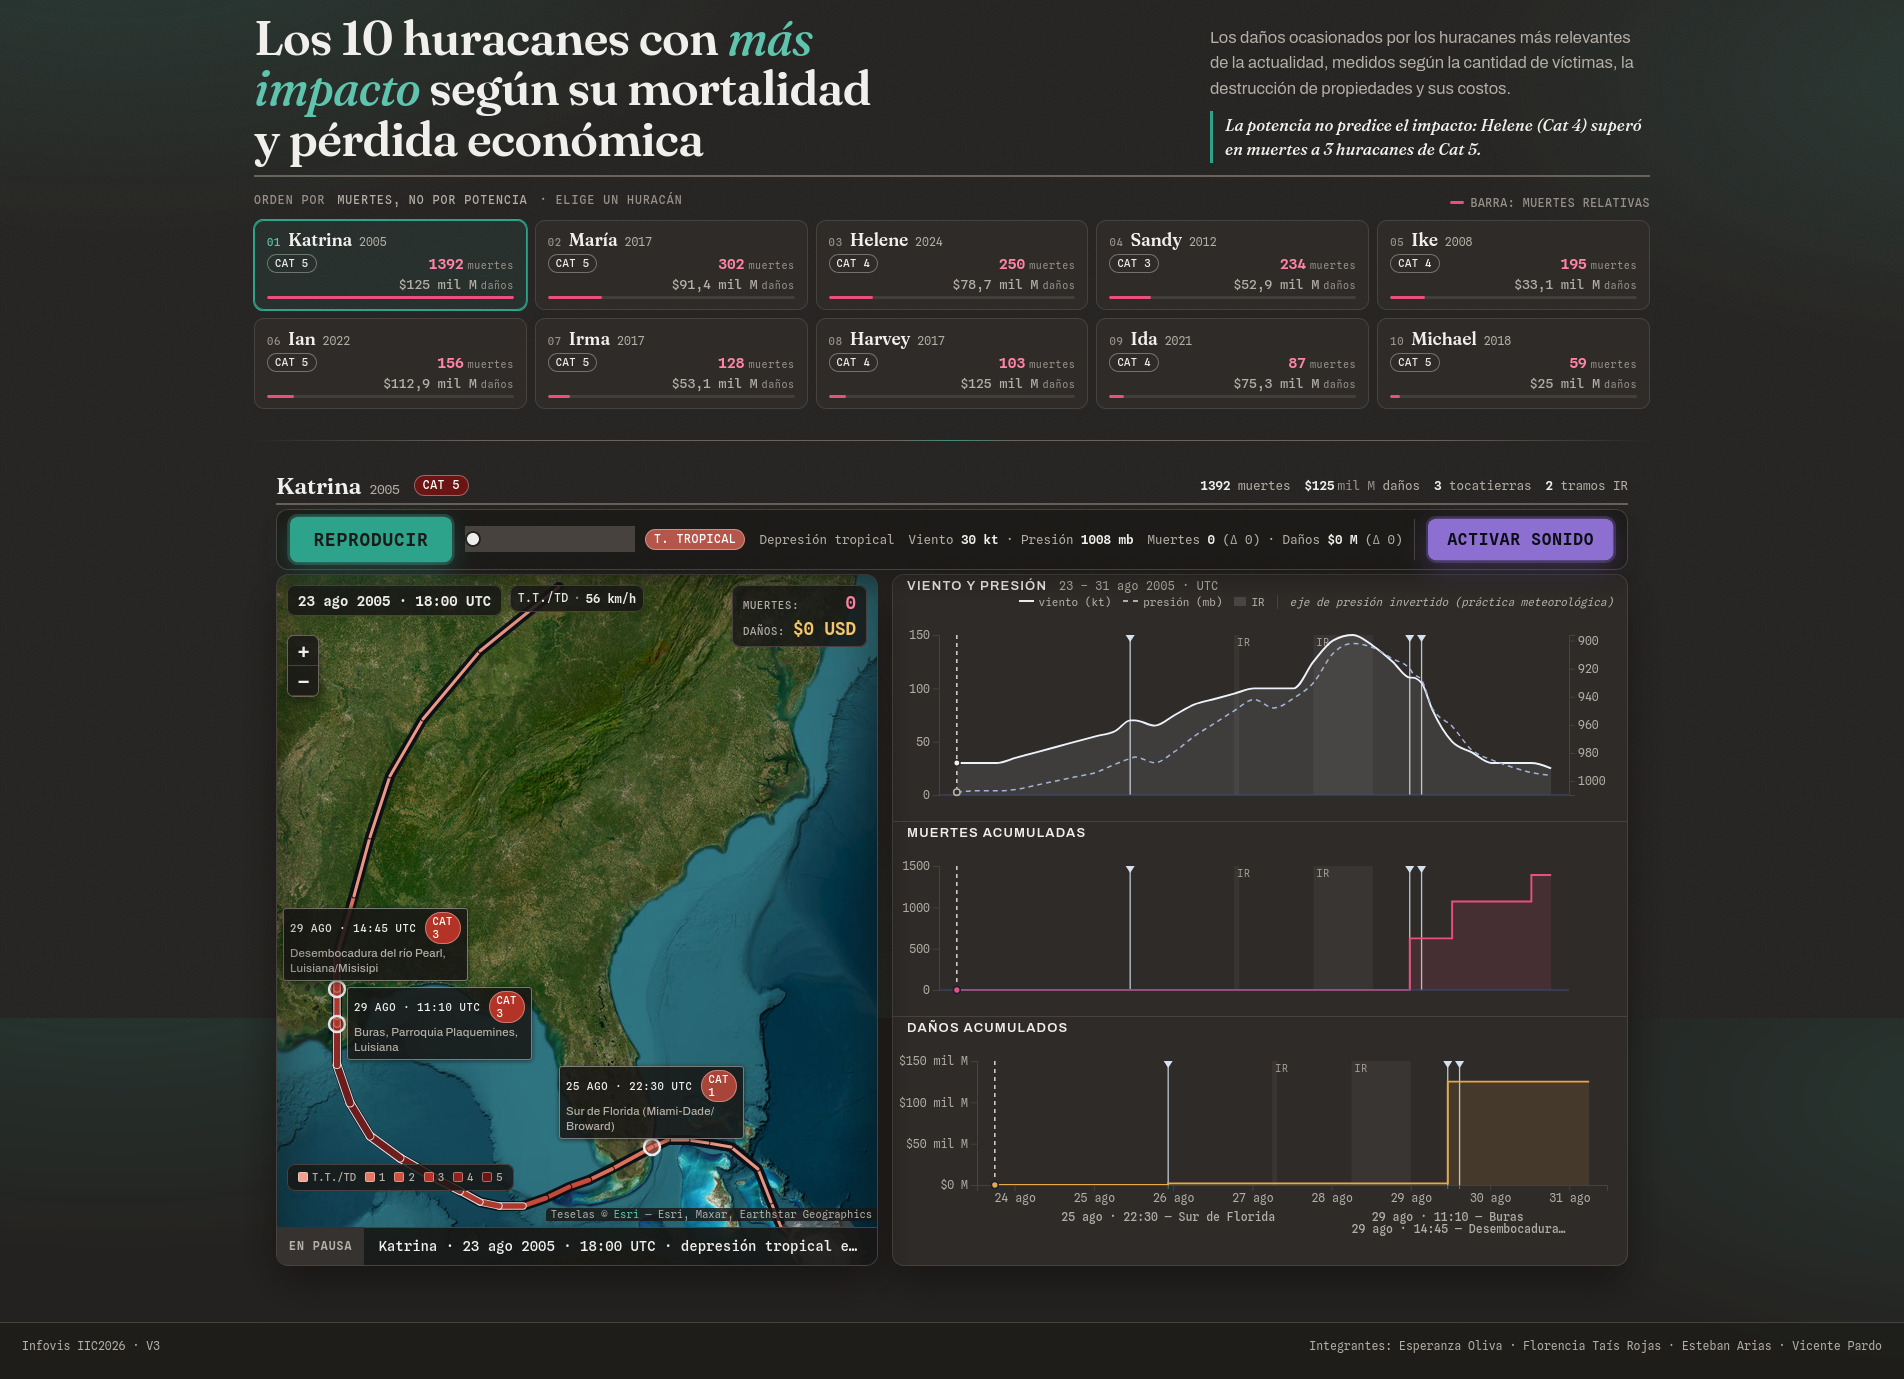
\includegraphics[width=0.88\textwidth]{figuras/captura_v3.png}
        \captionof{figure}{Interfaz refinada V3: ícono giratorio sobre la trayectoria, contador de impactos y daños sincronizados con los tocatierras.}
        \label{fig:v3}
    \end{center}

    \noindent\textbf{Qué cambió:}
    \begin{itemize}
        \item El ícono del huracán gira en sentido antihorario (ciclón del hemisferio norte) a velocidad proporcional al viento real, con el marcador reestructurado en dos capas para que el eje de giro quede clavado al punto exacto de la trayectoria (commit \texttt{3330309}).
        \item Deslizamiento interpolado del marcador entre fixes de 6~h durante la reproducción, sincronizado con el reloj UTC, y nuevos overlays del mapa: contador de muertes y daños acumulados e indicador de categoría y viento en km/h (commit \texttt{3330309}).
        \item Sincronización de la escalera de daños con los tocatierras (\texttt{sincronizar\_danos.py}): plana entre tocatierras y con salto exacto en cada uno, totales invariantes y proceso idempotente (commit \texttt{3330309}).
        \item Título y descripción editorales definitivos, enfocando el mensaje en el contraste entre mortalidad y costo material (commit \texttt{a3a2dab}).
        \item Corrección de los sistemas no ciclónicos: los estados LO/WV/DB (baja presión, onda tropical, disturbio) se conservan con su propia etiqueta («No tropical») en vez de colapsarse a «post-tropical», que narraba mal pasos como el de Harvey sobre Yucatán (commit \texttt{8814ab0}).
    \end{itemize}

    \vspace{0.15cm}
    \noindent\textbf{Por qué cambió — el rationale:}
    Movimiento con significado: la rotación del glifo codifica el viento real por un canal preatentivo y refuerza la lectura de intensidad sin añadir marcas; el giro se congela fuera de la reproducción y se anula con \textit{prefers-reduced-motion}. La sincronización de los daños con el tocatierra hace inmediata la lectura de la alineación temporal entre fenómeno y consecuencia. La corrección de los sistemas no ciclónicos impidió que estados ajenos a la escala Saffir–Simpson contaminaran la lectura posicional (Cleveland \& McGill: posición en escala común frente a estimaciones aproximadas).

    \vspace{0.15cm}
    \noindent\textbf{Qué se descartó:}
    Se descartó incluir sirenas de alarma o efectos estridentes tras comprobar que saturaban la mezcla acústica y distraían del seguimiento analítico de los gráficos.
\end{versionbox}

\vspace{0.4cm}

% ==============================================================================
% 8. R3 — REVISIÓN CON EL EQUIPO DOCENTE
% ==============================================================================
\begin{revisionbox}{R3 — Última Revisión con el Equipo Docente}{20 de octubre de 2026}
    \noindent\textbf{Fecha:} 20 de octubre de 2026.\\
    \textbf{Síntesis de lo discutido:} Se revisó la versión V3 previa a la entrega final. El profesor y los ayudantes elogiaron la profundidad de la investigación de datos, la fluidez interactiva y la sobriedad estética de la interfaz. La recomendación principal fue pulir la experiencia auditiva: eliminar cualquier residuo de zumbidos de alta frecuencia en el audio, balancear los volúmenes relativos para que el viento continúe siendo la columna vertebral de la atmósfera y optimizar la legibilidad del código.

    \vspace{0.15cm}
    \noindent\textbf{Decisiones tomadas (adoptado / descartado y por qué):}
    Se adoptó suprimir definitivamente el oscilador armónico de IR para erradicar cualquier molestia auditiva y proteger la inmersión del usuario. Se adoptó reestructurar y compactar \texttt{motor-audio.js} de 952 a 520 líneas, documentando detalladamente cada disparo acústico. Se descartó incorporar controles manuales de ecualización en la interfaz para no sobrecargar de mandos secundarios la vista principal.
\end{revisionbox}

\vspace{0.4cm}

% ==============================================================================
% 9. V4 — LA VERSIÓN FINAL
% ==============================================================================
\begin{versionbox}{V4 — La Versión Final}{20 de octubre de 2026 · Commits \texttt{792bb84}, \texttt{88e00e6}}
    \noindent\textbf{Evidencia visual y sonora:} Despliegue en producción en GitHub Pages (\textit{Figura~\ref{fig:v4}}). Paisaje sonoro equilibrado y depurado, con transiciones orgánicas y cero artefactos acústicos.

    \begin{center}
        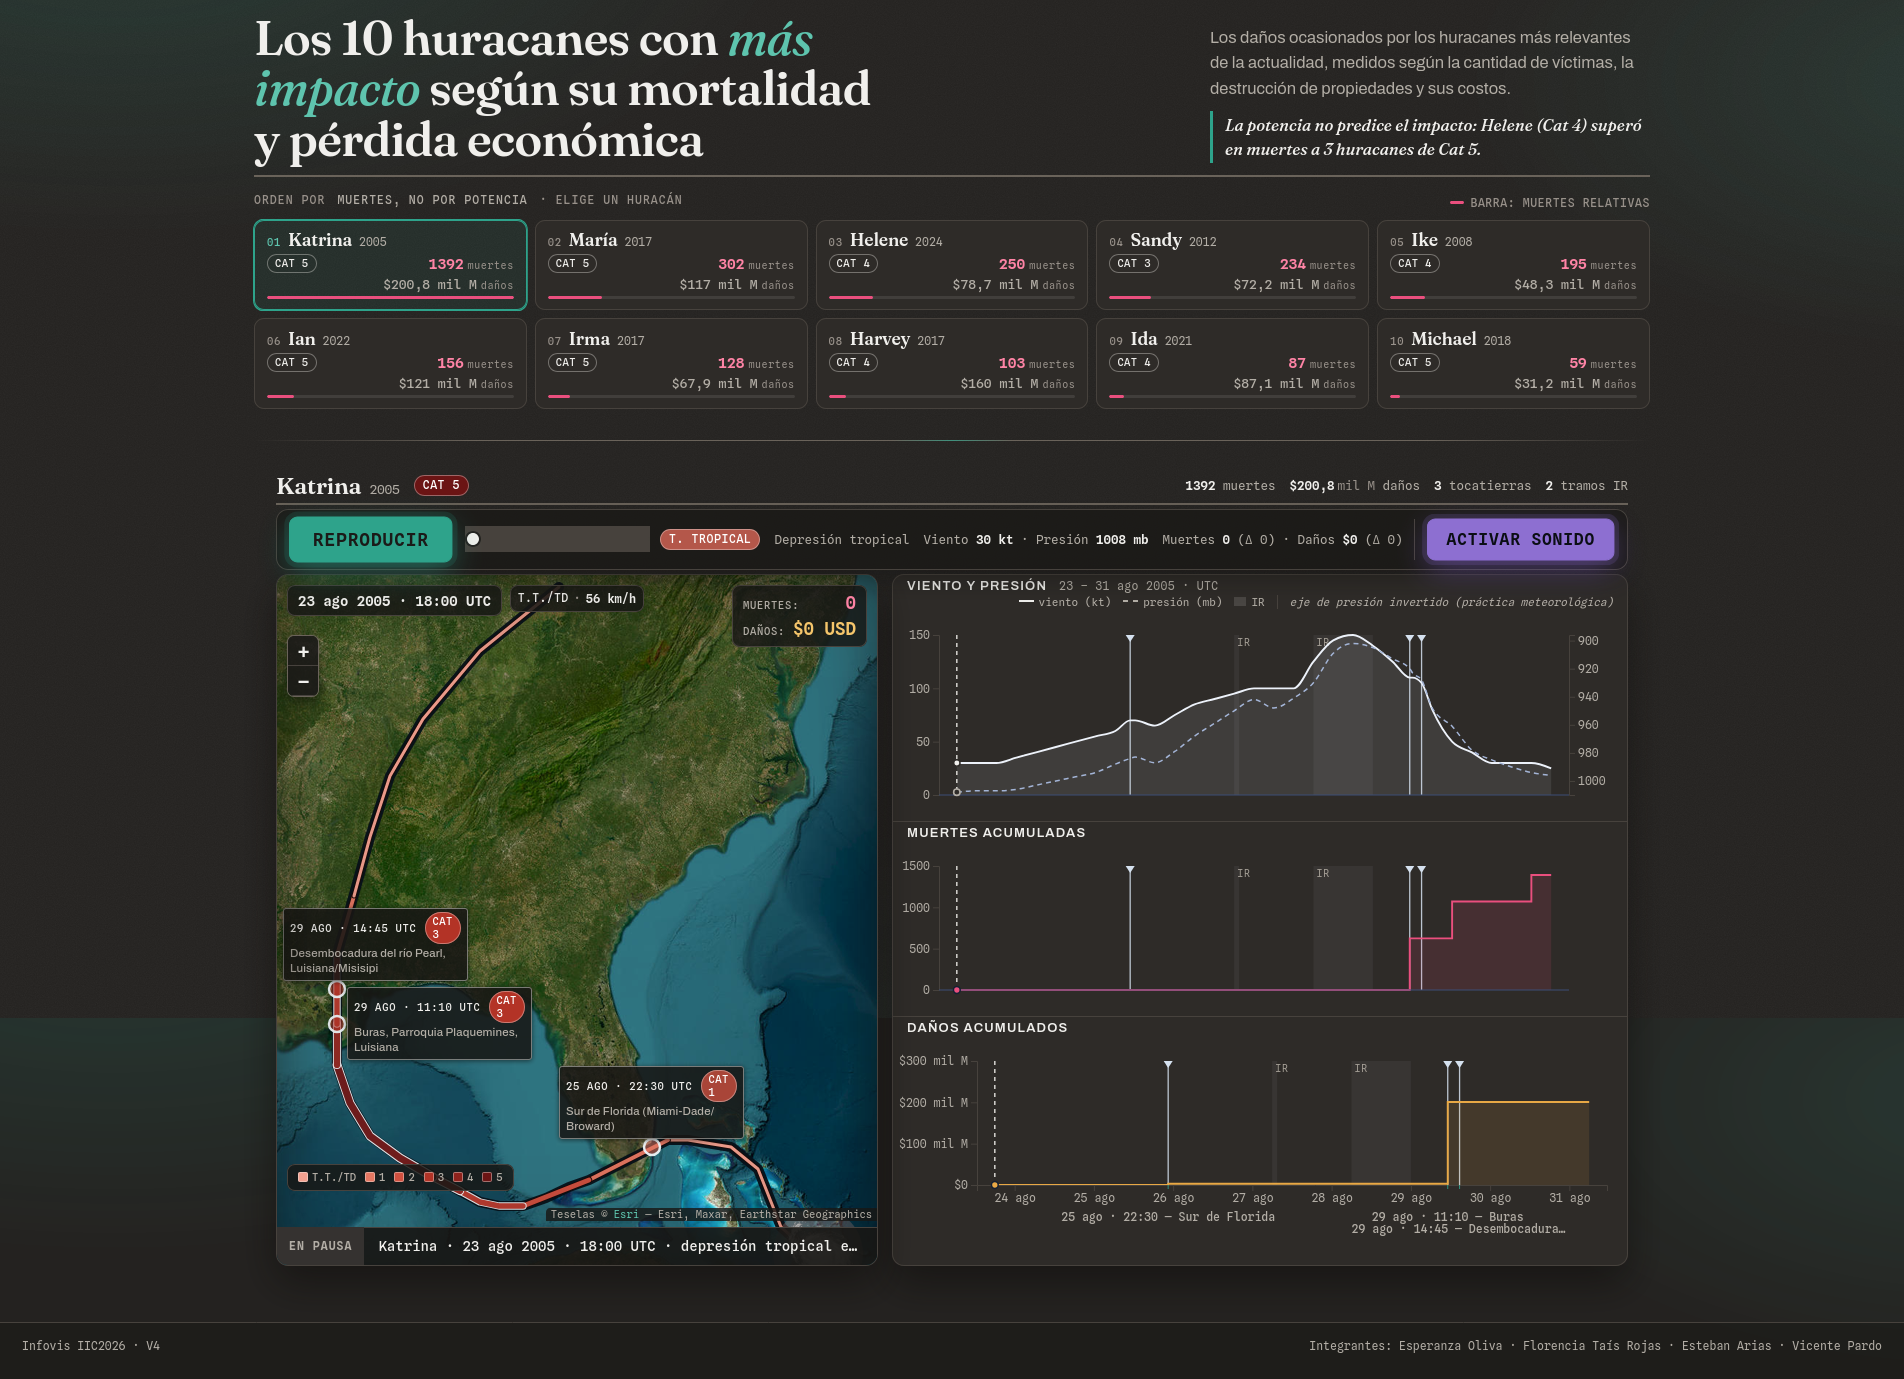
\includegraphics[width=0.92\textwidth]{figuras/captura_v4.png}
        \captionof{figure}{Versión final V4 en producción (\url{https://vpardos.github.io/vientovis/}).}
        \label{fig:v4}
    \end{center}

    \noindent\textbf{Qué cambió:}
    \begin{itemize}
        \item Erradicación completa del pitido agudo de IR (oscilador armónico); el dron sub-grave y el viento real dominan con nitidez el espectro (commit \texttt{88e00e6}).
        \item Refactorización arquitectónica de \texttt{motor-audio.js}: reducción de 952 a 520 líneas con constantes de mezcla explícitas (tabla de ganancia por categoría, ráfagas de daños al 75\,\%) y limpieza de nodos al terminar cada \textit{one-shot} (commit \texttt{88e00e6}).
        \item Pulido de \textit{bugs} latentes (commit \texttt{792bb84}): \textit{escape} seguro de HTML en todos los puntos de inyección, cancelación del temporizador de \textit{resize} al desmontar la tormenta y derivados (pico, tocatierras) computados una sola vez por montaje.
        \item Calibración final de balance dinámico: viento envolvente como base, tocatierra con pegada seca y ráfagas granulares escaladas logarítmicamente.
    \end{itemize}

    \vspace{0.15cm}
    \noindent\textbf{Por qué cambió — el rationale:}
    Principio de parsimonia y ley de Hick: la excelencia del diseño radica en eliminar todo elemento superfluo que no contribuya a la transmisión del mensaje. La depuración sonora elimina la fatiga auditiva identificada en las evaluaciones, permitiendo que el usuario explore pausadamente el desajuste temporal entre el pico meteorológico y la catástrofe social (como el rezago de Harvey, donde la lluvia acumulada y las inundaciones posteriores multiplicaron las víctimas días después del tocatierra).

    \vspace{0.15cm}
    \noindent\textbf{Qué se descartó:}
    Se descartaron efectos 3D y animaciones complejas de nubes que aumentaban el peso de carga y degradaban la legibilidad de las marcas de tocatierra y las trayectorias.
\end{versionbox}

\vspace{0.4cm}

% ==============================================================================
% 10. EL FEEDBACK AL OTRO GRUPO (R2)
% ==============================================================================
\section{El Feedback al Otro Grupo (Evaluación entre Pares · R2)}

\subsection{El Proyecto Evaluado}
Se evaluó el proyecto del Grupo 7, enfocado en visualizar la evolución de la red del Metro de Santiago y sus tiempos de desplazamiento entre comunas. La interfaz presentaba un mapa interactivo con isócronas de viaje y un gráfico de barras comparativo de afluencia por estación en horario punta.

\subsection{El Feedback que Dimos}
\begin{itemize}
    \item \textbf{Eje truncado en gráfico de afluencia:} Se observó que el eje de ordenadas comenzaba en 15.000 pasajeros en lugar de cero, exagerando visualmente diferencias mínimas entre estaciones centrales y violando el principio de proporcionalidad visual de Tufte.
    \item \textbf{Codificación de color errónea:} Utilizaban una rampa secuencial monocromática para representar líneas independientes del metro, lo que inducía una falsa jerarquía numérica; se recomendó usar paleta categórica de alto contraste.
    \item \textbf{Sonificación unidimensional:} El sonido se limitaba a modular el volumen con el número de pasajeros; se propuso codificar la congestión mediante cambios en el tempo rítmico y tono para una metáfora acústica más natural.
\end{itemize}

\subsection{Lo que nos Llevamos para Nuestro Propio Proyecto}
Reconocimos la importancia de explicitar inequívocamente las unidades de medida en cada tooltip y eje (kt, mb, USD, UTC). Comprobamos que en VientoVis algunas etiquetas de daños no aclaraban explícitamente si correspondían a miles de millones, lo que corregimos de inmediato.

\vspace{0.4cm}

% ==============================================================================
% 11. EVALUACIÓN CON USUARIOS — LA HOJA DEL OBSERVADOR
% ==============================================================================
\section{Evaluación con Usuarios — La Hoja del Observador}

\subsection{Identificación de la Sesión}
\textbf{Pensador:} Estudiante universitario ajeno al área de computación y meteorología (sin conocimiento previo del proyecto).\\
\textbf{Fecha y contexto:} 18 de octubre de 2026, sesión presencial con técnica de pensar en voz alta (\textit{thinking aloud}) sobre la versión V2 desplegada en ese momento.

\subsection{Bitácora de Observación (Citas Literales y Acciones)}
\begin{center}
\small
\begin{tabularx}{\textwidth}{lp{6.8cm}X}
\toprule
\textbf{Tiempo} & \textbf{Cita Literal del Pensador} & \textbf{Acción Concreta Observada} \\
\midrule
00:15 & «Veo fichas de huracanes ordenadas... Katrina y María están arriba con números gigantes.» & Recorre con el cursor la galería general sin hacer clic. \\
01:05 & «Al ponerle play el círculo avanza en el mar y el sonido empieza a rugir más fuerte.» & Hace clic en Katrina, activa el audio y pulsa Play. \\
01:50 & «¡Pum! Sonó un golpe seco cuando chocó la costa y la curva roja se disparó de golpe.» & Observa fijamente la línea de daños en el panel inferior. \\
02:40 & «En María el viento suena aterrador, pero hay un pitido agudo de fondo que me desconcentra.» & Cambia a María, arrastra el scrubber hacia atrás. \\
03:30 & «¿Las muertes son en el mismo momento que se cae la casa o cuentan las inundaciones de después?» & Pasa el cursor por el tooltip del punto de Puerto Rico. \\
\bottomrule
\end{tabularx}
\end{center}

\subsection{Qué Dijo del Sonido}
El pensador afirmó que el rugido del viento le permitía anticipar la peligrosidad de la tormenta sin necesidad de fijar la vista en las cifras de nudos. Manifestó que el golpe de tocatierra le producía un sobresalto coherente con el impacto costero. Sin embargo, criticó tajantemente el silbido de alta frecuencia en intensificación rápida, describiéndolo como molesto y artificial.

\subsection{Heurísticas que Fallaron (Zuk-Carpendale)}
\begin{itemize}
    \item \textbf{El sonido no se entiende sin explicación previa:} El armónico agudo de IR se percibió como un pitido irritante o interferencia de audio en lugar de una alerta deliberada de intensificación meteorológica.
    \item \textbf{Falta de contexto en la métrica:} Inicialmente dudó sobre si la mortalidad correspondía a muertes directas o indirectas, requiriendo mayor claridad en las notas metodológicas.
\end{itemize}

\subsection{Las Tres Preguntas de Cierre}
\begin{enumerate}
    \item \textbf{¿Dónde se atascó más tiempo?:} Intentando descifrar el motivo del zumbido agudo en la reproducción de María y Harvey.
    \item \textbf{¿Qué hipótesis dijo en voz alta y resultó equivocada?:} Asumió que el momento de mayor viento siempre coincidía con el momento de más muertes, sorprendiéndose al ver que en tormentas de lluvia masiva las muertes ocurren días después.
    \item \textbf{¿Qué cambio concreto sale de esta sesión?:} Eliminar por completo el oscilador armónico agudo de IR en el motor sonoro e incorporar notas contextuales claras en las fichas sobre muertes directas e indirectas.
\end{enumerate}

\subsection{Efecto Visible en el Proceso}
Este hallazgo motivó la reescritura directa de \texttt{motor-audio.js} en la V4, erradicando el oscilador armónico molesto y consolidando una atmósfera sonora centrada en el viento real.

\vspace{0.4cm}

% ==============================================================================
% 12. CHECKLIST Y DECLARACIÓN DE CUMPLIMIENTO
% ==============================================================================
\section{Checklist de Cumplimiento de la Entrega}

\begin{metabox}
\begin{itemize}
    \item[\checkmark] \textbf{Ciclo de diseño evidente:} Se documentan 4 versiones completas con evolución justificada y trazable en el repositorio.
    \item[\checkmark] \textbf{Tipos de visualización adecuados:} Ejes temporales compartidos con crosshair y mapa geográfico sincronizado para análisis multivariable.
    \item[\checkmark] \textbf{Sin errores comunes:} Cero ejes truncados en magnitudes lineales; escala de presión invertida declarada y justificada.
    \item[\checkmark] \textbf{Mantra de Shneiderman:} Visión general en galería $\rightarrow$ selección y filtrado $\rightarrow$ detalles a demanda mediante tooltips y fichas.
    \item[\checkmark] \textbf{Sonificación multivariable:} Parámetros acústicos dirigidos por variables reales (viento, presión, tocatierra, víctimas y daños).
    \item[\checkmark] \textbf{Revisiones y feedback documentados:} Registro riguroso de R1, R2, R3, feedback entregado al Grupo 7 y hoja de observación con usuarios.
\end{itemize}
\end{metabox}

\end{document}
